% =============================================================
%  PREÁMBULO
% =============================================================

\documentclass[12pt,a4paper]{article}

% --- Codificación y fuente ---
\usepackage{lmodern}           % Estabiliza métricas base (fix glue units)
\usepackage[utf8]{inputenc}
\usepackage[T1]{fontenc}
\usepackage[spanish,es-tabla]{babel}
\usepackage{csquotes}  % Requerido por biblatex + babel

% --- Tipografía ---
\usepackage[sfdefault]{FiraSans}  % Fuente moderna sin conflictos con pgfplots
\usepackage{setspace}
\onehalfspacing

% --- Márgenes ---
\usepackage{geometry}
\geometry{
    a4paper,
    left=3cm,
    right=2.5cm,
    top=2.5cm,
    bottom=2.5cm,
    headheight=14.5pt  % Requerido por fancyhdr
}

% --- Matemáticas ---
\usepackage{amsmath}
\usepackage{amssymb}
\usepackage{amsthm}
\newtheorem{teorema}{Teorema}[section]
\newtheorem{definicion}{Definición}[section]

% --- Gráficos y figuras ---
\usepackage{graphicx}
\usepackage{float}
\usepackage{subcaption}
\usepackage{rotating}

% --- Tablas ---
\usepackage{tabularx}
\usepackage{booktabs}
\usepackage{array}
\usepackage{multirow}

% --- Código (Matlab) ---
\usepackage{listings}
\usepackage{xcolor}
\lstset{
    language=Matlab,
    basicstyle=\ttfamily\small,
    keywordstyle=\color{blue}\bfseries,
    commentstyle=\color{gray}\itshape,
    stringstyle=\color{orange},
    backgroundcolor=\color{lightgray!20},
    frame=single,
    breaklines=true,
    captionpos=b,
    showstringspaces=false
}

% --- Plots ---
\usepackage{pgfplots}
\pgfplotsset{compat=1.18}

% --- Miscelánea ---
\usepackage{enumerate}
\usepackage{eurosym}
\usepackage{ragged2e}

% --- Encabezados y pie de página ---
\usepackage{fancyhdr}
\pagestyle{fancy}
\fancyhf{}  % Limpia todos los campos
\fancyhead[L]{\small\itshape Diseño de Circuitos Impresos}
\fancyhead[R]{\small\itshape UPV · ETSIT}
\fancyfoot[C]{\thepage}
\renewcommand{\headrulewidth}{0.4pt}
\renewcommand{\footrulewidth}{0pt}

% --- Bibliografía ---
\usepackage[backend=biber]{biblatex}
\addbibresource{mybibliography.bib}

% --- Hipervínculos (siempre al final del preámbulo) ---
\usepackage[
    colorlinks = true,
    linkcolor  = {blue!60!black},
    citecolor  = {blue!60!black},
    urlcolor   = {blue!60!black}
]{hyperref}

% =============================================================

\begin{document}

% --- PORTADA ---
\begin{titlepage}
    \centering

    % Logo UPV
    
\includegraphics[width=0.60\textwidth]{Imagenes/190470_190083_keystone_profile_school_logo-marca_UPV_principal_negro300.png}

    \vspace{1.2cm}

    {\large Escuela Técnica Superior de Ingeniería de Telecomunicación}\\[0.2cm]
    {\large Universitat Politècnica de València}

    \vspace{1.8cm}
    \rule{\linewidth}{0.8pt}\\[0.5cm]

    {\Huge\bfseries Trabajo Final\\[0.4cm]
    Diseño de Circuitos Impresos}\\[0.5cm]

    \rule{\linewidth}{0.8pt}

    \vspace{1.2cm}

    {\large\itshape Informe de diseño}\\[0.3cm]
    {\normalsize Descripción del diseño, justificación de decisiones\\
    y resultados de simulación y análisis}

    \vfill

    \begin{tabular}{rl}
        \textbf{Autores:}         & Joan San Bartolomé \\
                                  & Raúl Tarazona      \\[0.6cm]
        \textbf{Asignatura:}      & Diseño de Circuitos Impresos \\[0.6cm]
        \textbf{Curso académico:} & 2025--2026
    \end{tabular}

    \vspace{1.5cm}

\end{titlepage}

% Activa encabezados a partir de aquí (la portada usa su propio estilo vacío)
\pagestyle{fancy}

\newpage
\thispagestyle{plain}  % ToC sin encabezado, solo número de página
\tableofcontents

\newpage

\section{Introducción}

El presente trabajo aborda el diseño, desarrollo y validación de una tarjeta de circuito impreso (PCB) funcional y fabricable basada en el microcontrolador de alto rendimiento STM32F746ZG. Tomando como referencia la plataforma de desarrollo comercial ST NUCLEO-F746ZG, el objetivo principal es adaptar y optimizar su arquitectura original en Altium Designer. Para ello, se simplifica el sistema mediante la eliminación de componentes redundantes y de evaluación (como el depurador integrado ST-LINK/V2-1) y se integran de forma nativa periféricos y acondicionadores de señal adaptados a aplicaciones específicas de control y conectividad.

Una de las decisiones clave de simplificación consiste en sustituir el programador/depurador ST-LINK embebido por un conector de depuración y programación SWD (Serial Wire Debug) estándar de 10 pines y paso de 100 mils. Esta decisión reduce sustancialmente el área de la placa y el consumo de potencia, permitiendo realizar la depuración mediante un programador externo o puenteando las señales desde el propio bloque ST-LINK de una placa NUCLEO comercial.

Entre los requisitos y capacidades integradas en este diseño se encuentran:
\begin{itemize}
    \item \textbf{Conectividad de red:} Interfaz Ethernet a través de un conector RJ45 de montaje inserción con LEDs de estado y magnéticos externos.
    \item \textbf{Comunicación serie y buses diferenciales:} Un puerto Micro-USB y dos transceptores CAN con opción de terminación de línea seleccionable mediante puente.
    \item \textbf{Adquisición de datos analógicos:} Dos canales de acondicionamiento de señal para entradas analógicas en rango de $0-10\text{ V}$, reduciéndolas y adaptándolas al rango de $0-3.3\text{ V}$ compatible con el ADC del microcontrolador.
    \item \textbf{Almacenamiento no volátil:} Una memoria SPI Flash de 2 MB para el almacenamiento de datos o firmware.
    \item \textbf{Expansión:} Un conector con 16 señales GPIO de propósito general protegidas y desacopladas.
\end{itemize}

El diseño físico de la tarjeta se ha planteado en una tecnología de 4 capas para garantizar la integridad de las señales de alta velocidad (RMII de Ethernet, USB y CAN) y optimizar la Red de Distribución de Alimentación (PDN). Se configuran planos internos dedicados para masa (GND) y alimentación (PWR, este último partido para abastecer los diferentes niveles de tensión). El diseño cumple estrictamente las directivas de fabricación especificadas por el fabricante \textit{Lab Circuits}, restringiendo el grosor total de la placa a un máximo de $1.6\text{ mm}$ y aplicando reglas de ruteado originales para distanciar este prototipo del formato de evaluación de ST.

\section{Especificaciones de la placa}
La placa cuenta con distintos elementos que hacen que sea funcional para muchas situaciones y entornos, a continuación, se verán los diferentes elementos y funcionalidades de la placa a la vez que su construcción.

\subsection{Microcontrolador}

El cerebro de la tarjeta es el microcontrolador de muy alto rendimiento \textbf{STM32F746ZGT6}, basado en el núcleo ARM Cortex-M7 con FPU de 32 bits. Este dispositivo opera con un rango de tensión de alimentación de $1.7\text{ V}$ a $3.6\text{ V}$ y alcanza una frecuencia de reloj máxima de $216\text{ MHz}$. Dispone de $1\text{ MB}$ de memoria Flash, $320\text{ KB}$ de memoria SRAM (incluyendo memorias TCM de baja latencia) y se presenta en un encapsulado \textbf{LQFP144 de 144 pines}.

Para garantizar la estabilidad temporal del sistema, el diseño incorpora dos osciladores externos:
\begin{itemize}
    \item \textbf{Oscilador de Alta Velocidad (HSE):} Un cristal de cuarzo de $8\text{ MHz}$ conectado a los pines \texttt{PH0} y \texttt{PH1}, esencial para alimentar el PLL principal y derivar los relojes de alta precisión necesarios para Ethernet (RMII) y USB.
    \item \textbf{Oscilador de Baja Velocidad (LSE):} Un cristal de $32.768\text{ kHz}$ en los pines \texttt{PC14} y \texttt{PC15} dedicado al reloj de tiempo real (RTC) y estados de bajo consumo.
\end{itemize}

El arranque de la placa (\textit{boot}) se gestiona de forma manual mediante el pin \texttt{BOOT0}: por defecto se mantiene a nivel bajo ($0$) con una resistencia de pulso hacia abajo (\textit{pull-down}) de $10\text{ k}\Omega$ para iniciar desde la memoria Flash interna, pero cuenta con un pulsador físico que lo conecta a $3.3\text{ V}$ (a través de una resistencia en serie de $100\,\Omega$) para forzar el arranque en modo \textit{System Memory} (cargador de arranque por defecto de ST). La programación y depuración de la placa se realizan a través de un puerto SWD simplificado empleando los pines dedicados \texttt{PA13} (SWDIO) y \texttt{PA14} (SWCLK), además de la línea de reinicio activa a nivel bajo \texttt{NRST}.

\subsection{ADC y Acondicionamiento de Señal Analógica}

La placa incorpora dos canales independientes para la adquisición de señales analógicas industriales en un rango de $0-10\text{ V}$. Dado que el rango de entrada del ADC del microcontrolador está limitado a $0-3.3\text{ V}$ (tensión de referencia analógica), hemos diseñado una etapa de acondicionamiento para atenuar, filtrar y adaptar la impedancia de la señal.

\begin{figure}[H]
    \centering
    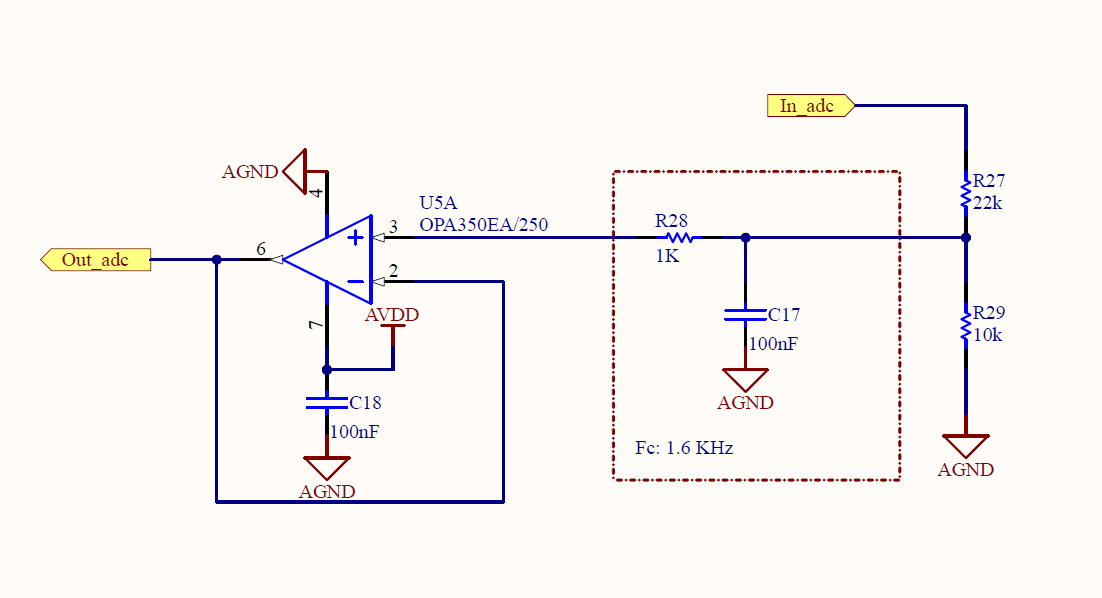
\includegraphics[width=0.75\linewidth]{Imagenes/ADC_esquema.png}
    \caption{Esquemático de la etapa de acondicionamiento analógico de entrada.}
    \label{fig:adc_esquema}
\end{figure}

El circuito de acondicionamiento de cada canal consta de las siguientes etapas:
\begin{enumerate}
    \item \textbf{Divisor de tensión atenuador:} Para adaptar la señal al rango del microcontrolador, hemos diseñado un divisor resistivo con $R_{18} = 22\text{ k}\Omega$ y $R_{19} = 10\text{ k}\Omega$. Este divisor atenúa la tensión máxima de entrada de $10\text{ V}$ a un valor seguro de $3.125\text{ V}$, protegiendo el pin de entrada y aprovechando el $95\%$ del rango dinámico del ADC.
    \item \textbf{Filtro paso bajo (Anti-aliasing):} Conectado a la entrada no inversora del amplificador operacional, este filtro RC pasivo está formado por $R_{20} = 1\text{ k}\Omega$ y $C_{12} = 100\text{ nF}$. Fija la frecuencia de corte en $f_c \approx 1.59\text{ kHz}$, adecuada para eliminar interferencias electromagnéticas y ruido de alta frecuencia de sensores industriales.
    \item \textbf{Buffer de adaptación de impedancia:} Se implementa mediante el amplificador operacional de alta precisión \textbf{OPA350EA/250} en configuración de seguidor de tensión (ganancia unidad). Al estar colocado tras el filtro, este buffer aprovecha la impedancia de entrada casi infinita de sus terminales para no cargar el filtro RC, ofreciendo a su vez una salida de muy baja impedancia idónea para alimentar el circuito de muestreo del ADC del microcontrolador ($R_{ADC} \approx 6\text{ k}\Omega$) sin errores de carga.
\end{enumerate}

Para evitar oscilaciones térmicas y consumos indeseados, el segundo canal del amplificador operacional (\texttt{U5B}), al no ser utilizado en este bloque jerárquico, se ha estabilizado conectándolo en modo seguidor con su pin no inversor unido a la masa analógica (\texttt{AGND}).

\subsubsection{Pines asignados para el ADC}

Las señales acondicionadas se conectan a los siguientes pines del microcontrolador:

\begin{table}[H]
\centering
\begin{tabular}{|c|c|l|}
\hline
\textbf{Señal} & \textbf{Pin MCU} & \textbf{Función del Periférico} \\ \hline
ADC\_CH1 & PB0 & Canal de conversión analógico-digital (ADC12\_IN8) \\ \hline
ADC\_CH2 & PB1 & Canal de conversión analógico-digital (ADC12\_IN9) \\ \hline
\end{tabular}
\caption{Asignación de pines para los canales analógicos.}
\label{tab:adc_pines}
\end{table}



\subsection{Interfaz de Comunicación CAN (Controller Area Network)}

El estándar CAN es un protocolo robusto de comunicación diferencial, idóneo para entornos industriales debido a su elevada inmunidad al ruido electromagnético. Hemos implementado en la placa dos nodos CAN independientes (\texttt{CAN1} y \texttt{CAN2}) utilizando una arquitectura jerárquica idéntica.

\begin{figure}[H]
    \centering
    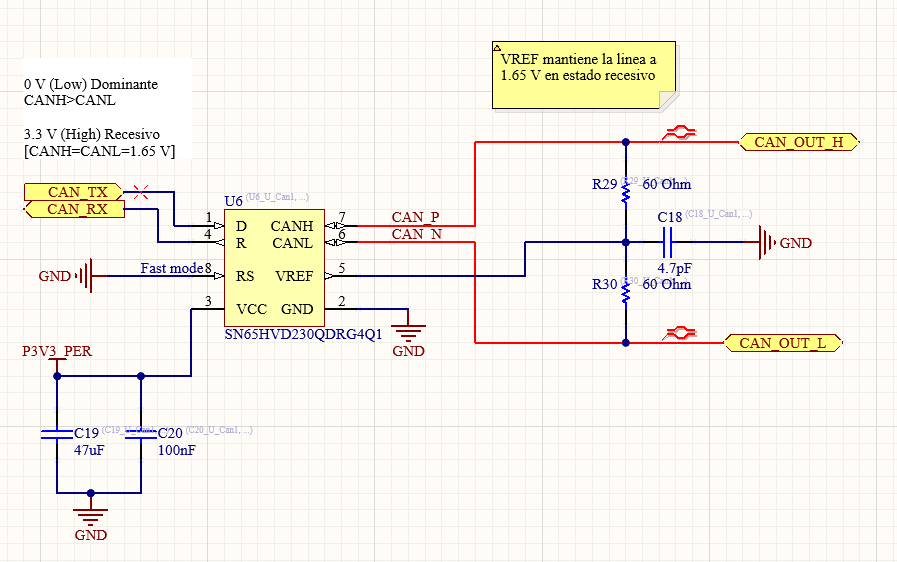
\includegraphics[width=0.75\linewidth]{Imagenes/CAN_esquema.png}
    \caption{Esquemático de la etapa del transceptor CAN e inmunidad contra ESD.}
    \label{fig:can_esquema}
\end{figure}

Para cada canal hemos tomado las siguientes decisiones de diseño de hardware:
\begin{enumerate}
    \item \textbf{Transceptor de baja potencia a $3.3\text{ V}$:} Hemos integrado el chip \textbf{SN65HVD230Q}, el cual opera directamente con la tensión lógica del microcontrolador ($3.3\text{ V}$), eliminando la necesidad de emplear desplazadores de nivel de tensión que habrían encarecido y complicado el ruteado.
    \item \textbf{Terminación de línea dividida (Split Termination):} En lugar de una única resistencia de $120\,\Omega$, hemos implementado de forma integrada una terminación dividida compuesta por dos resistencias de $60\,\Omega$ en serie, conectando el punto común de unión a masa a través de un condensador de $4.7\text{ nF}$. Esta configuración actúa como un filtro paso bajo para el ruido en modo común, disipando las interferencias de alta frecuencia a tierra sin alterar la impedancia diferencial del bus. Esta red forma parte del ruteado permanente de la tarjeta.
    \item \textbf{Control de pendiente (RS Pin):} El pin de control de modo/pendiente (\texttt{RS}) del transceptor se conecta a masa a través de una resistencia de $0\,\Omega$ por defecto. Esto configura el transceptor en modo de alta velocidad (\textit{High-Speed Mode}). Sin embargo, la huella permite sustituir esta resistencia por un valor mayor ($10\text{ k}\Omega$ a $100\text{ k}\Omega$) para pasar a modo de control de pendiente y limitar la velocidad de transición de los flancos en caso de no cumplir con los ensayos de compatibilidad electromagnética (EMI).
    \item \textbf{Protección contra transitorios (ESD):} Hemos colocado un diodo de protección ESD bidireccional específico para CAN en encapsulado SOT-23 (\textbf{PESD2CAN}) lo más cerca posible del conector físico de salida para derivar descargas electrostáticas y transitorios directamente a la masa del sistema.
\end{enumerate}

\subsubsection{Pines asignados para el bus CAN}

La interfaz lógica entre el microcontrolador y los transceptores se realiza a través de las siguientes líneas:

\begin{table}[H]
\centering
\begin{tabular}{|c|c|l|l|}
\hline
\textbf{Periférico} & \textbf{Pin MCU} & \textbf{Señal Lógica} & \textbf{Función} \\ \hline
\multirow{2}{*}{CAN1} & PD0 & CAN1\_RX & Recepción de datos lógicos del transceptor \\ \cline{2-4} 
                      & PD1 & CAN1\_TX & Transmisión de datos lógicos al transceptor \\ \hline
\multirow{2}{*}{CAN2} & PB5 & CAN2\_RX & Recepción de datos lógicos del transceptor \\ \cline{2-4} 
                      & PB6 & CAN2\_TX & Transmisión de datos lógicos al transceptor \\ \hline
\end{tabular}
\caption{Asignación de pines de comunicación lógica para los controladores CAN.}
\label{tab:can_pines}
\end{table}

\subsection{Interfaz Micro-USB}

Hemos integrado un puerto Micro-USB de tipo AB (receptáculo \textbf{Molex 475900001}) para dotar a la tarjeta de conectividad de datos (USB 2.0 Full-Speed a $12\text{ Mbps}$) y permitir la alimentación del sistema a través del bus VBUS del host.

\begin{figure}[H]
    \centering
    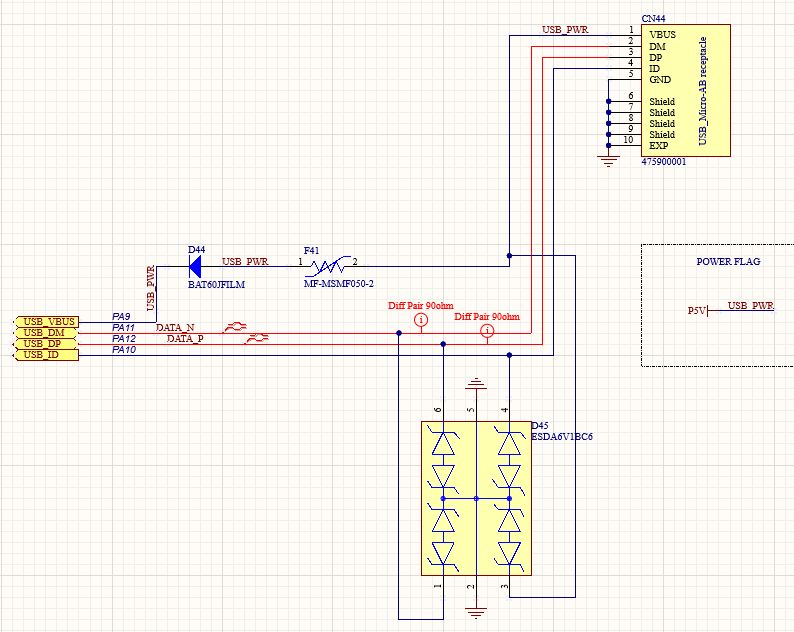
\includegraphics[width=0.75\linewidth]{Imagenes/USB_esquema.png}
    \caption{Esquemático de la etapa del conector USB con sus elementos de protección y filtrado.}
    \label{fig:usb_esquema}
\end{figure}

El diseño físico y eléctrico de esta interfaz se fundamenta en las siguientes decisiones de hardware:
\begin{enumerate}
    \item \textbf{Adaptación de impedancia diferencial:} Las líneas de datos $D+$ y $D-$ se rutan como par diferencial directamente desde el conector hacia los pines del microcontrolador, sin resistencias serie de terminación externas. Hemos aprovechado que el transceptor Full-Speed integrado en el microcontrolador STM32F746ZGT6 cuenta con una impedancia de salida adaptada por hardware. El par se ha diseñado para presentar una impedancia diferencial de \textbf{$90\,\Omega \pm 10\%$}.
    \item \textbf{Protección contra descargas electrostáticas (ESD):} Para proteger las líneas de datos de transitorios de alta velocidad sin degradar la señal por efecto capacitivo, hemos colocado el circuito integrado de capacitancia ultra-baja ($C_{in} \approx 1\text{ pF}$) \textbf{USBLC6-4SC6} lo más cerca posible del conector físico. Las pistas del par de datos se rutan pasando directamente a través de las patillas del integrado para evitar stubs en el diseño de la pista.
    \item \textbf{Seguridad de alimentación (VBUS):} La entrada de alimentación desde el puerto USB (\texttt{USB\_PWR}) cuenta con dos niveles de protección activa:
        \begin{itemize}
            \item Un fusible rearmable PTC de $0.5\text{ A}$ (\textbf{MF-MSMF050-2}) para proteger al puerto del host frente a cortocircuitos o sobrecorrientes en nuestra placa.
            \item Un diodo Schottky \textbf{BAT60JFILM} que previene corrientes de retorno inversas hacia el host cuando la placa se alimenta mediante otra fuente de alimentación externa.
        \end{itemize}
    \item \textbf{Sensado de VBUS:} La línea VBUS se conecta al pin de entrada analógica/digital \texttt{PA9} del microcontrolador a través de una resistencia en serie de $10\text{ k}\Omega$. Aprovechando que el pin \texttt{PA9} es tolerante a $5\text{ V}$, esta resistencia actúa como un limitador de corriente para salvaguardar la entrada ante picos de tensión o transitorios en la línea de alimentación USB, permitiendo al firmware detectar la presencia del host y gestionar el stack de comunicaciones de forma dinámica.
\end{enumerate}

\subsubsection{Cálculo de Impedancia del Par Diferencial USB}

Para asegurar la integridad de la señal en el bus de datos USB, hemos realizado el cálculo geométrico del par diferencial utilizando el motor de cálculo \textit{SIMBEOR} integrado en el gestor de pila de capas (\textit{Layer Stack Manager}) de Altium Designer. 

Tomando como base la pila de capas de $1.6\text{ mm}$ de \textit{Lab Circuits}, los parámetros geométricos y eléctricos que definen el par diferencial de datos USB ($90\,\Omega$) se muestran en la Tabla~\ref{tab:usb_diffpair_params}:

\begin{table}[H]
\centering
\small
\begin{tabular}{|l|c|}
\hline
\textbf{Parámetro del Par Diferencial} & \textbf{Valor de Diseño} \\ \hline
Impedancia Objetivo ($Z_{diff}$) & $90\,\Omega$ \\ \hline
Tolerancia de Diseño & $15\%$ \\ \hline
Ancho de Pista ($W1$ / $W2$) & $0.19\text{ mm}$ ($\approx 7.5\text{ mils}$) \\ \hline
Separación de Pistas (Gap, $G$) & $0.15\text{ mm}$ ($\approx 6\text{ mils}$) \\ \hline
Grosor de la Máscara de Soldadura ($C1$ / $C2$) & $0.0254\text{ mm}$ ($1\text{ mil}$) \\ \hline
\textbf{Impedancia Diferencial Calculada ($Z_{diff}$)} & $\mathbf{94.91\,\Omega}$ \\ \hline
Desviación de Impedancia Obtenida & $5.46\%$ (dentro de límites) \\ \hline
Retardo de Propagación (Delay) & $5.90\text{ ns/m}$ \\ \hline
\end{tabular}
\caption{Parámetros de diseño calculados para el par diferencial USB de 90 Ohm.}
\label{tab:usb_diffpair_params}
\end{table}

\subsubsection{Pines asignados para el puerto USB}

El mapeo de pines entre el microcontrolador y el conector USB se detalla a continuación:

\begin{table}[H]
\centering
\small
\begin{tabularx}{\textwidth}{|c|c|l|X|}
\hline
\textbf{Señal} & \textbf{Pin MCU} & \textbf{Señal Lógica} & \textbf{Función del Periférico} \\ \hline
USB\_VBUS & PA9 & OTG\_FS\_VBUS & Entrada de detección de presencia de tensión de VBUS \\ \hline
USB\_ID & PA10 & OTG\_FS\_ID & Línea de detección de modo Host/Device (OTG) \\ \hline
USB\_DM & PA11 & OTG\_FS\_DM & Línea de datos diferencial negativa (D-) \\ \hline
USB\_DP & PA12 & OTG\_FS\_DP & Línea de datos diferencial positiva (D+) \\ \hline
\end{tabularx}
\caption{Asignación de pines para la interfaz Micro-USB.}
\label{tab:usb_pines}
\end{table}

\subsection{Sistema de Alimentación y Red de Distribución de Potencia (PDN)}

La tarjeta se alimenta primariamente a través del puerto Micro-USB ($5\text{ V}$). Dado que la electrónica principal (núcleo del microcontrolador, transceptores y periféricos) funciona a un nivel nominal de $3.3\text{ V}$, hemos implementado una etapa de regulación lineal y una red de desacoplo distribuida (PDN) para asegurar el suministro limpio y estable de energía.

\begin{figure}[H]
    \centering
    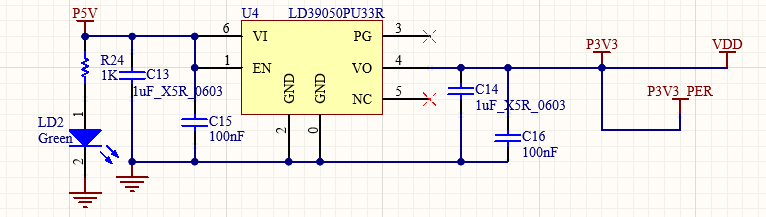
\includegraphics[width=0.75\linewidth]{Imagenes/Alimentacion_squema.png}
    \caption{Esquema de la etapa del regulador LDO de 3.3V y filtrado de alimentación.}
    \label{fig:alimentacion_esquema}
\end{figure}

Las decisiones de diseño tomadas para la red de alimentación son las siguientes:
\begin{enumerate}
    \item \textbf{Regulador LDO de alta eficiencia:} Hemos seleccionado el regulador de bajo descarte (LDO) \textbf{LD39050PU33R} de STMicroelectronics en encapsulado DFN-6, capaz de suministrar hasta $500\text{ mA}$ con una excelente relación de rechazo al rizado (PSRR). Este regulador incorpora una patilla de \textit{Power Good} (PG) para verificar la correcta estabilidad de la tensión y un pin de habilitación (\texttt{EN}) para control lógico. Su salida está estabilizada mediante una red de condensadores de $1\,\mu\text{F}$ y $100\text{ nF}$.
    \item \textbf{Desacoplo local del microcontrolador:} Para minimizar la inductancia del bucle de retorno y atenuar el ruido de conmutación de alta frecuencia, hemos colocado un condensador de desacoplo cerámico de $100\text{ nF}$ (encapsulado 0402) inmediatamente adyacente a cada uno de los 12 pines de alimentación digital \texttt{VDD} del microcontrolador.
    \item \textbf{Condensadores de almacenamiento masivo (Bulk):} Para responder ante transitorios de corriente rápidos del núcleo a $216\text{ MHz}$, hemos distribuido estratégicamente condensadores bulk en los extremos de la placa: un condensador de $4.7\,\mu\text{F}$ en las proximidades del pin 95 y otro de $10\,\mu\text{F}$ (X5R, 0805) junto al pin 72.
    \item \textbf{Regulación interna del núcleo (VCAP):} El regulador interno de $1.2\text{ V}$ para el núcleo digital del microcontrolador requiere estabilidad externa obligatoria. Para ello, hemos conectado dos condensadores cerámicos de bajo ESR de $2.2\,\mu\text{F}$ desde los pines dedicados \texttt{VCAP\_1} y \texttt{VCAP\_2} directamente a masa.
    \item \textbf{Aislamiento del dominio analógico ($V_{DDA}$ / $V_{REF+}$):} Para evitar el acoplamiento de ruido digital de alta frecuencia en las medidas del ADC, hemos aislado la alimentación analógica mediante una perla de ferrita de muy baja resistencia en continua (\textbf{Murata BLM18PG121SN1D}), acompañada de un desacoplo local de $1\,\mu\text{F}$ y $100\text{ nF}$. La baja DCR ($< 50\text{ m}\Omega$) garantiza una caída de tensión insignificante ($< 0.15\text{ mV}$), preservando la precisión de las lecturas analógicas.
\end{enumerate}

\subsubsection{Pines de alimentación del microcontrolador}

La distribución física de las patillas de alimentación y masa del microcontrolador STM32F746ZGT6 se describe en la siguiente tabla:

\begin{table}[H]
\centering
\small
\begin{tabular}{|l|c|p{7.5cm}|}
\hline
\textbf{Dominio de Potencia} & \textbf{Símbolo Pin} & \textbf{Pines Físicos (LQFP144)} \\ \hline
Alimentación Digital & VDD & 16, 30, 39, 52, 62, 72, 84, 95, 108, 121, 131, 144 \\ \hline
Masa Común & VSS & 15, 31, 38, 51, 61, 71, 83, 94, 107, 120, 130, 143 \\ \hline
Alimentación Analógica & VDDA & 33 \\ \hline
Masa Analógica & VSSA & 32 \\ \hline
Tensión de Referencia Analógica & VREF+ / VREF- & 35 / 34 \\ \hline
Alimentación de Batería & VBAT & 6 \\ \hline
Condensadores del Regulador Núcleo & VCAP\_1 / VCAP\_2 & 71 / 106 \\ \hline
\end{tabular}
\caption{Pines físicos de alimentación y referencia en encapsulado LQFP144.}
\label{tab:alimentacion_pines}
\end{table}

\subsection{Interfaz de Red Ethernet}

Hemos incorporado conectividad Ethernet 10/100Base-TX mediante el uso del microcontrolador en modo MAC y un transceptor de capa física (PHY) externo de bajo consumo \textbf{LAN8742A-CZ-TR} en encapsulado QFN-24. La conexión física se realiza a través de un conector RJ45 con transformador magnético integrado (\textbf{KRJ-CB4.2GYZNL}).

El diseño de esta etapa se basa en las siguientes decisiones técnicas de hardware:
\begin{enumerate}
    \item \textbf{Uso de interfaz RMII (Reduced Media Independent Interface):} Para reducir el número de patillas necesarias en el microcontrolador de 17 (modo MII) a 9, hemos configurado la comunicación en modo RMII. La señal de reloj de referencia de $50\text{ MHz}$ (\texttt{RMII\_REF\_CLK}) es generada por el propio PHY a partir de un cristal local de $25\text{ MHz}$ y se introduce en el pin \texttt{PA1} del microcontrolador.
    \item \textbf{Aislamiento galvánico bajo los magnéticos:} Para evitar el acoplamiento de ruido electromagnético de modo común procedente de la línea de red cableada hacia los planos internos de alimentación y masa de la placa, hemos definido un área de exclusión de cobre (\textit{keep-out}) en todas las capas de la PCB por debajo de la zona ocupada por los transformadores magnéticos del conector RJ45.
    \item \textbf{Protección contra transitorios:} Hemos colocado un array de diodos de capacitancia ultra-baja \textbf{USBLC6-4SC6} adyacente a las líneas diferenciales del conector para filtrar picos de ESD antes de que alcancen el lado del transceptor.
\end{enumerate}

\subsubsection{Cálculo de Impedancia del Par Diferencial Ethernet}

Las líneas del bus MDI que enlazan el transceptor PHY con el conector RJ45 (\texttt{TX+/TX-} y \texttt{RX+/RX-}) requieren un control de impedancia diferencial de **$100\,\Omega$**. Hemos calculado la geometría del par en base a la pila de capas de $1.6\text{ mm}$ de \textit{Lab Circuits} utilizando el motor de cálculo \textit{SIMBEOR} de Altium Designer. Los valores resultantes se detallan en la Tabla~\ref{tab:ethernet_diffpair_params}:

\begin{table}[H]
\centering
\small
\begin{tabular}{|l|c|}
\hline
\textbf{Parámetro del Par Diferencial} & \textbf{Valor de Diseño} \\ \hline
Impedancia Objetivo ($Z_{diff}$) & $100\,\Omega$ \\ \hline
Tolerancia de Diseño & $10\%$ \\ \hline
Ancho de Pista ($W1$ / $W2$) & $0.182\text{ mm}$ ($\approx 7.2\text{ mils}$) \\ \hline
Separación de Pistas (Gap, $G$) & $0.180\text{ mm}$ ($\approx 7.1\text{ mils}$) \\ \hline
Grosor de la Máscara de Soldadura ($C1$ / $C2$) & $0.0254\text{ mm}$ ($1\text{ mil}$) \\ \hline
\textbf{Impedancia Diferencial Calculada ($Z_{diff}$)} & $\mathbf{99.99\,\Omega}$ \\ \hline
Desviación de Impedancia Obtenida & $0.01\%$ \\ \hline
Retardo de Propagación (Delay) & $5.91\text{ ns/m}$ \\ \hline
\end{tabular}
\caption{Parámetros de diseño calculados para el par diferencial Ethernet de 100 Ohm.}
\label{tab:ethernet_diffpair_params}
\end{table}

\subsubsection{Pines asignados para el bus Ethernet}

Las señales lógicas del bus de control y datos RMII están distribuidas de acuerdo con la siguiente tabla:

\begin{table}[H]
\centering
\small
\begin{tabularx}{\textwidth}{|l|c|X|}
\hline
\textbf{Señal RMII} & \textbf{Pin MCU} & \textbf{Función de la Señal} \\ \hline
RMII\_REF\_CLK & PA1 & Reloj de referencia de 50 MHz para sincronización \\ \hline
RMII\_MDIO & PA2 & Gestión de datos bidireccional (SMI) \\ \hline
RMII\_MDC & PC1 & Reloj de la interfaz de gestión (SMI) \\ \hline
RMII\_CRS\_DV & PA7 & Detección de portadora y validación de datos recibidos \\ \hline
RMII\_RXD0 & PC4 & Línea 0 de recepción de datos \\ \hline
RMII\_RXD1 & PC5 & Línea 1 de recepción de datos \\ \hline
RMII\_TX\_EN & PG11 & Habilitación de transmisión de datos \\ \hline
RMII\_TXD0 & PG13 & Línea 0 de transmisión de datos \\ \hline
RMII\_TXD1 & PB13 & Línea 1 de transmisión de datos \\ \hline
nRST (PHY) & Pin 25 & Línea de reinicio por hardware del microcontrolador (NRST) \\ \hline
\end{tabularx}
\caption{Asignación de pines para la interfaz Ethernet en modo RMII.}
\label{tab:ethernet_pines}
\end{table}


\subsection{Conectores}
Además de las interfaces de comunicación específicas, hemos integrado conectores de expansión y terminales de conexión externa para interactuar con señales analógicas y digitales del sistema:

\begin{enumerate}
    \item \textbf{Conector de Expansión General (CN41):} Se trata de un conector macho de cabezal de $18\times2$ vías (paso de $2.54\,\text{mm}$) que expone un total de 16 líneas GPIO generales del microcontrolador (pertenecientes a los puertos C, D y G) y 4 líneas correspondientes a las interfaces USART6 y USART7.
    \item \textbf{Conector de Depuración SWD (CN42):} Un cabezal de $6\times1$ vías utilizado para la programación y depuración del STM32F746ZG, exponiendo las líneas de depuración esenciales (SWCLK, SWDIO, SWO y el pin de reinicio NRST).
    \item \textbf{Terminales de Entrada Analógica (J41):} Un bloque de bornes de tornillo Weidmüller, modelo \textbf{1845040000} (paso de $3.50\,\text{mm}$ y entrada a $90^\circ$), que proporciona una conexión segura para las dos entradas analógicas acondicionadas de $0-10\,\text{V}$.
    \item \textbf{Conectores de Bus CAN (J42 y J43):} Conectores macho de 2 pines JST tipo \textbf{B2B-EH-A(LF)(SN)} para las conexiones físicas de los buses de comunicación CAN1 y CAN2.
\end{enumerate}

\subsubsection{Estrategia de Protección de Entradas/Salidas}
Para garantizar la inmunidad del microcontrolador frente a eventos externos de sobretensión y descargas electrostáticas (ESD), hemos diseñado e implementado un esquema de protección multietapa para todas las líneas de entrada y salida expuestas:
\begin{itemize}
    \item \textbf{Protección ESD Primaria (TVS Diodes):} Inmediatamente después del conector físico, hemos colocado matrices de diodos de supresión de tensiones transitorias (TVS) de 4 canales bidireccionales, modelo \textbf{ESDA6V1BC6} (D46, D47, D48 y D49). Estos dispositivos poseen una tensión de ruptura de $6.1\,\text{V}$, ideal para proteger pines tolerantes a $5\,\text{V}$ sin distorsionar señales de datos. Su ubicación física adyacente al conector y su baja inductancia de conexión a masa aseguran que los transitorios se deriven a tierra de forma instantánea.
    \item \textbf{Protección de Línea CAN:} Los puertos J42 y J43 disponen de diodos de protección TVS específicos de bus CAN de alta inmunidad y baja capacitancia modelo \textbf{PESD2CANFD24V-TR} (D44 y D45), situados en paralelo con las líneas diferenciales CAN\_H y CAN\_L.
    \item \textbf{Limitación de Corriente Secundaria (Resistencias Serie):} Entre las matrices TVS y los pines de entrada del microcontrolador, hemos introducido resistencias de protección en serie. Para las líneas de propósito general expuestas en CN41, hemos seleccionado resistencias de $100\,\Omega$ (R58 a R65 para el puerto D, y R69 a R73 para los puertos G/C). Estas resistencias limitan la corriente transitoria residual que pudiera llegar al microcontrolador a un nivel seguro inferior al límite de conducción de los diodos de fijación (clamping diodes) internos del STM32F746ZG ($I_{IN} < 10\,\text{mA}$).
    \item \textbf{Líneas de Depuración SWD:} Las señales del conector CN42 (SWCLK, SWDIO, SWO y NRST) se conectan al MCU mediante resistencias en serie de $22\,\Omega$ (R43, R44, R45 y R46), las cuales reducen sobreoscilaciones (overshoot/undershoot) y previenen reflexiones de alta frecuencia causadas por la impedancia de los cables de programación.
\end{itemize}

La topología de ruteado implementada respeta estrictamente la secuencia física: \textbf{[Conector Exterior]} $\rightarrow$ \textbf{[Diodo TVS ESDA6V1BC6 / PESD2CANFD]} $\rightarrow$ \textbf{[Resistencia Serie]} $\rightarrow$ \textbf{[Pin del MCU]}.

\subsubsection{Asignación de Pines del Conector General (CN41)}

La Tabla~\ref{tab:conectores_pines} muestra el mapeo detallado de cada pin del conector CN41, incluyendo las señales de alimentación y tierra correspondientes:

\begin{table}[H]
\centering
\small
\begin{tabularx}{\textwidth}{|l|c|X|l|}
\hline
\textbf{Señal del Esquema} & \textbf{Pin MCU} & \textbf{Función Asignada} & \textbf{Pin Conector CN41} \\ \hline
GND & -- & Plano de Masa de Referencia & 1, 2, 7, 8, 13, 14, 21, 22, 29, 30, 35, 36 \\ \hline
P5V & -- & Alimentación +5 V (desde USB) & 3, 4 \\ \hline
P3V3 & -- & Alimentación +3.3 V Regulada & 5, 6 \\ \hline
PinG4 & PG4 & I/O de Propósito General & 9 \\ \hline
PinC6 & PC6 & I/O de Propósito General & 10 \\ \hline
PinG5 & PG5 & I/O de Propósito General & 11 \\ \hline
PinG8 & PG8 & I/O de Propósito General & 12 \\ \hline
PinG2 & PG2 & I/O de Propósito General & 15 \\ \hline
PinG7 & PG7 & I/O de Propósito General & 16 \\ \hline
PinG3 & PG3 & I/O de Propósito General & 17 \\ \hline
PinG6 & PG6 & I/O de Propósito General & 18 \\ \hline
PinD14 & PD14 & I/O de Propósito General & 19 \\ \hline
PinD11 & PD11 & I/O de Propósito General & 20 \\ \hline
PinD15 & PD15 & I/O de Propósito General & 23 \\ \hline
PinD10 & PD10 & I/O de Propósito General & 24 \\ \hline
PinD12 & PD12 & I/O de Propósito General & 25 \\ \hline
PinD9 & PD9 & I/O de Propósito General & 26 \\ \hline
PinD13 & PD13 & I/O de Propósito General & 27 \\ \hline
PinD8 & PD8 & I/O de Propósito General & 28 \\ \hline
USART7\_TX & PE8 & Transmisión USART7 / GPIO & 31 \\ \hline
USART6\_TX & PG14 & Transmisión USART6 / GPIO & 32 \\ \hline
USART7\_RX & PE7 & Recepción USART7 / GPIO & 33 \\ \hline
USART6\_RX & PG9 & Recepción USART6 / GPIO & 34 \\ \hline
\end{tabularx}
\caption{Distribución de pines del conector de expansión general (CN41) y su asignación en el microcontrolador.}
\label{tab:conectores_pines}
\end{table}

\subsection{Memoria Flash}
Para el almacenamiento de firmware auxiliar, archivos de configuración o parámetros no volátiles del sistema, hemos incorporado una memoria Flash externa de tipo SPI NOR de $4\,\text{Mbit}$ ($512\,\text{KB}$), modelo \textbf{SST25VF040B-50-4I-S2AF} (encapsulado SOIC-8). Este chip se comunica con el microcontrolador a través del bus serie síncrono SPI2.

\subsubsection{Criterios de Diseño para la Integridad de la Señal SPI}
Debido a la alta frecuencia de conmutación del bus SPI (que puede operar hasta $50\,\text{MHz}$), hemos tomado las siguientes precauciones en el diseño del circuito:
\begin{itemize}
    \item \textbf{Amortiguación del Reloj (SCK):} Hemos colocado una resistencia amortiguadora en serie de $33\,\Omega$ (R32) en la línea de reloj (SPI\_CLK / SCK), ubicada en la cercanía física del microcontrolador (emisor). Esto permite controlar la impedancia de salida del driver, reducir la velocidad de subida del flanco (slew rate) y prevenir rebotes o sobreoscilaciones destructivas que podrían causar falsas transiciones de reloj en la memoria.
    \item \textbf{Resistencias de Pull-Up en Control:} Hemos colocado resistencias de pull-up de $10\,\text{k}\Omega$ a la línea de $3.3\,\text{V}$ (R31) en las líneas de control activas a nivel bajo: \textbf{CE\#} (Chip Enable), \textbf{WP\#} (Write Protect) y \textbf{HOLD\#} (Hold). Estas resistencias de pull-up aseguran que durante el arranque del microcontrolador (cuando sus pines se encuentran en alta impedancia), la memoria permanezca deshabilitada y protegida contra cualquier escritura o borrado accidental.
    \item \textbf{Desacoplo local:} Hemos colocado un condensador de desacoplo de $100\,\text{nF}$ (C61) en paralelo al terminal de alimentación VDD (Pin 8) a masa, ubicado lo más próximo posible al integrado.
\end{itemize}

La asignación de pines y conexiones físicas para la memoria Flash SPI se detallan en la Tabla~\ref{tab:flash_pines}:

\begin{table}[H]
\centering
\small
\begin{tabularx}{\textwidth}{|l|c|c|X|}
\hline
\textbf{Señal del Esquema} & \textbf{Pin Memoria (SOIC-8)} & \textbf{Pin MCU} & \textbf{Descripción y Detalles de Diseño} \\ \hline
SPI\_CS / CE\# & Pin 1 & PB12 & Habilitación de chip (Chip Enable). Dispone de un pull-up de $10\,\text{k}\Omega$ a 3.3V. \\ \hline
SPI\_MISO / SO & Pin 2 & PB14 & Salida de datos serie (Serial Data Output). Conexión directa a MISO del bus SPI2. \\ \hline
WP\# & Pin 3 & -- & Entrada de protección contra escritura. Conectada a +3.3 V mediante pull-up de $10\,\text{k}\Omega$. \\ \hline
GND / VSS & Pin 4 & -- & Terminal de referencia de masa. \\ \hline
SPI\_MOSI / SI & Pin 5 & PB15 & Entrada de datos serie (Serial Data Input). Conexión directa a MOSI del bus SPI2. \\ \hline
SPI\_CLK / SCK & Pin 6 & PB10 & Reloj serie (Serial Clock). Conectado mediante resistencia amortiguadora serie de $33\,\Omega$. \\ \hline
HOLD\# & Pin 7 & -- & Entrada de pausa temporal de bus. Conectada a +3.3 V mediante pull-up de $10\,\text{k}\Omega$. \\ \hline
VDD & Pin 8 & -- & Alimentación a +3.3 V, desacoplada localmente con condensador cerámico de $100\,\text{nF}$. \\ \hline
\end{tabularx}
\caption{Mapeo de pines y criterios de conexión para la memoria Flash SPI externa SST25VF040B.}
\label{tab:flash_pines}
\end{table}



\subsection{Stack-up}

Para poder hacer un buen ajuste de impedancias dentro de la PCB es muy importante el diseño adecuado del Stack-up, en esta PCB hay líneas diferenciales de CAN ($120\Omega$), Ethernet ($100\Omega$), USB ($90\Omega$). También la PCB cuenta con una impedancia Singel ended de 50 $\Omega$ para todas las líneas de alimentación y señales no tan críticas.

La PCB consta de 4 capas, 2 para señales (top y bottom) y 2 para alimentaciones (3.3V y GND). Como consideraciones a tener en cuenta es que la PCB debe de ser aproximadamente de 1.6mm de espesor, en concreto esta PCB es de 1.62mm, un valor muy próximo a esos 1.6mm. En lo que respecta al espesor del cobre, como no es una PCB de potencia (donde va a pasar gran cantidad de corriente) por lo que en este caso se ha puesto en capas de señal media onza y en alimentación, una onza. Aquí está el diseño del stack-up:

\begin{figure}[H]
    \centering
    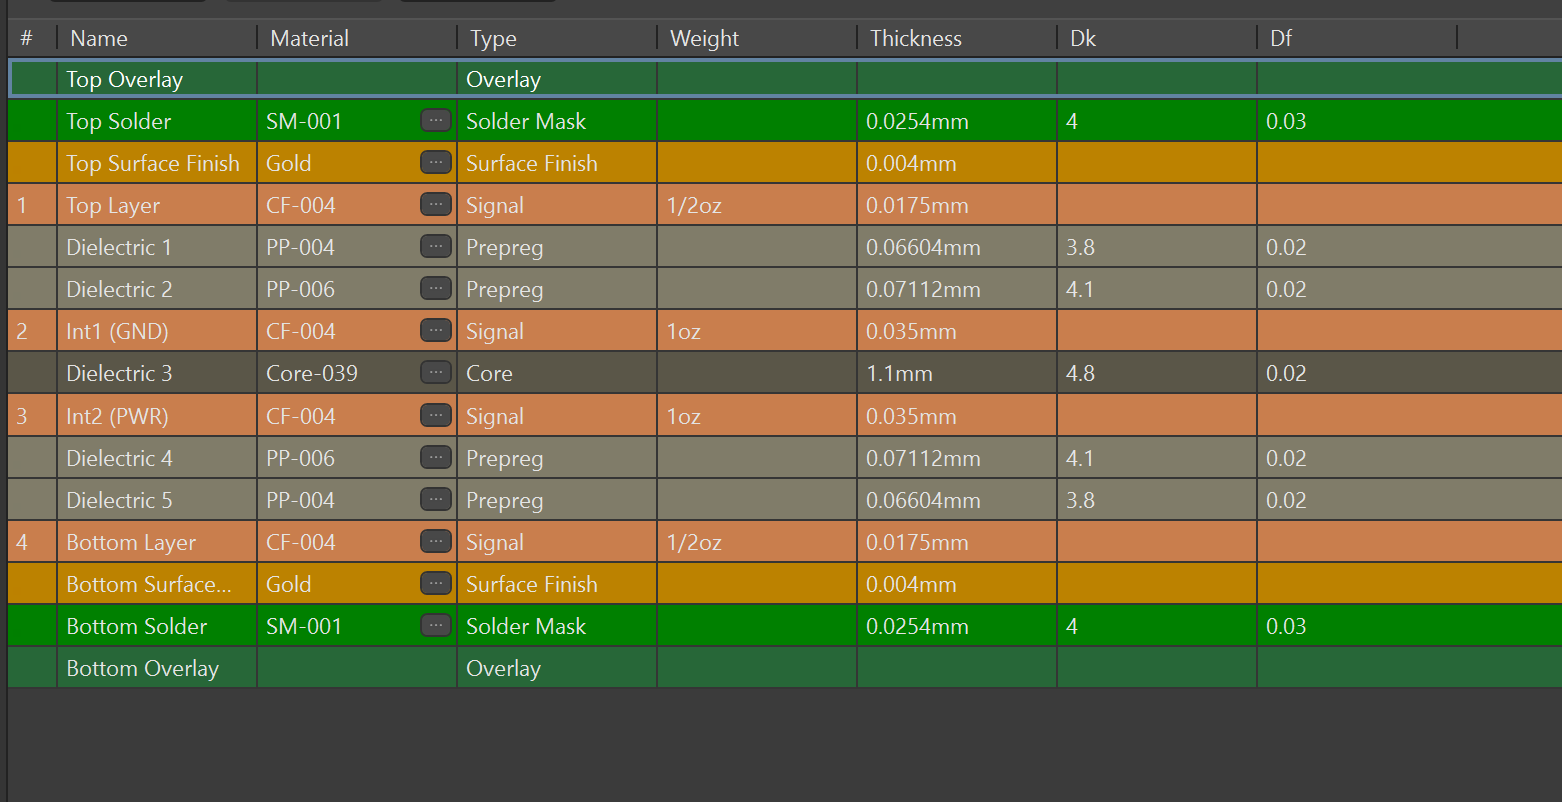
\includegraphics[width=1\linewidth]{Imagenes/Captura_stackup.png}
    \caption{Propuesta de Stack-Up 4 capas}
    \label{fig:stackup}
\end{figure}

\subsubsection{Impedancias de los diferentes buses de comunicación y pistas}

Ahora se va a poner una tabla con los valores de impedancia obtenidos con este stack-up.

\begin{table}[H]
\centering
\footnotesize
\caption{Comparación entre impedancias ideales y obtenidas}
\label{tab:impedancias}
\begin{tabular}{|p{2.8cm}|p{2.8cm}|c|c|c|}
\hline
\textbf{Comunicación} &
\textbf{Tipo de comunicación} &
\textbf{Impedancia ideal} &
\textbf{Impedancia real} &
\textbf{Variación} \\ \hline

CAN &
Diferencial &
$120\,\Omega$ &
$113\,\Omega$ &
$5.89$\,\% \\ \hline

Ethernet &
Diferencial &
$100\,\Omega$ &
$104\,\Omega$ &
$4.3$\,\% \\ \hline

USB &
Diferencial &
$90\,\Omega$ &
$94.45\,\Omega$ &
$4.95$\,\% \\ \hline

Resto de pistas &
Single-ended &
$50\,\Omega$ &
$53.65\,\Omega$ &
$7.3$\,\% \\ \hline

\end{tabular}
\end{table}


\section{Reflexiones}

Para comprobar el buen rutado de la placa se va a realizar un análisis para la integridad de señal en las pistas del PCB para ver si tanto el rutado, las consideraciones y los cálculos son correctos para evitar reflexiones en las pistas que pueden afectar al buen funcionamiento del PCB.

\subsection{CAN}

\begin{figure}[H]
    \centering
    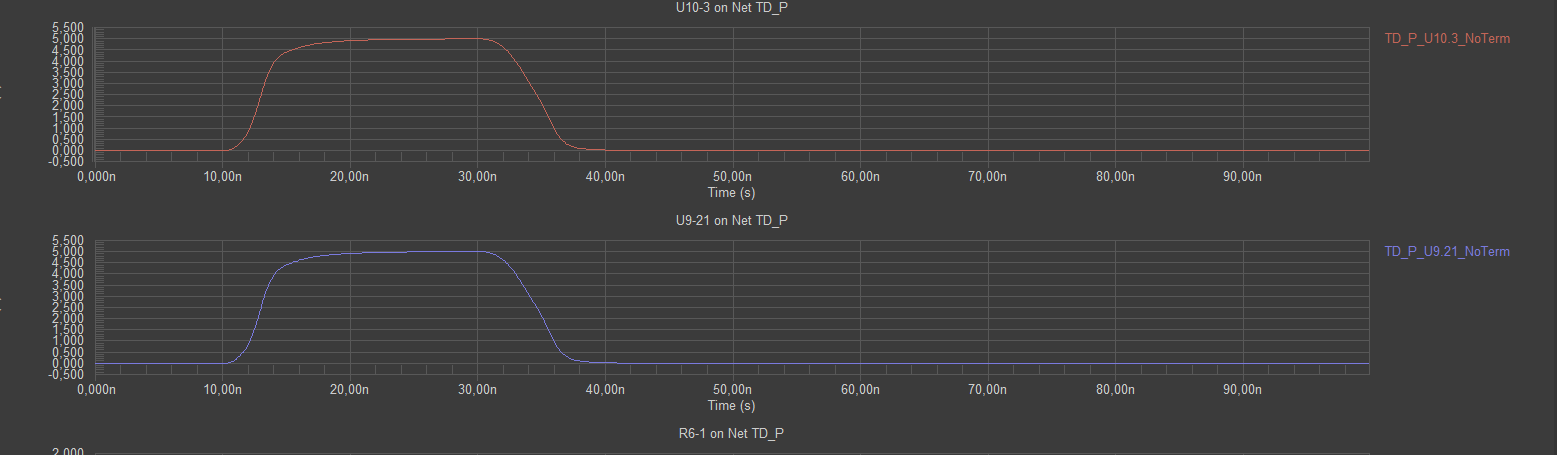
\includegraphics[width=1\linewidth]{Imagenes/Reflexiones CAN.png}
    \caption{Reflexiones Can}
    \label{fig:reflexiones_can}
\end{figure}

Como se observa en la imagen las gráficas de las reflexiones del bus CAN no se aprecian reflexiones, lo que es positivo porque eso quiere decir que existe una buena adaptación de impedancias.


\subsection{USB}

\begin{figure}[H]
    \centering
    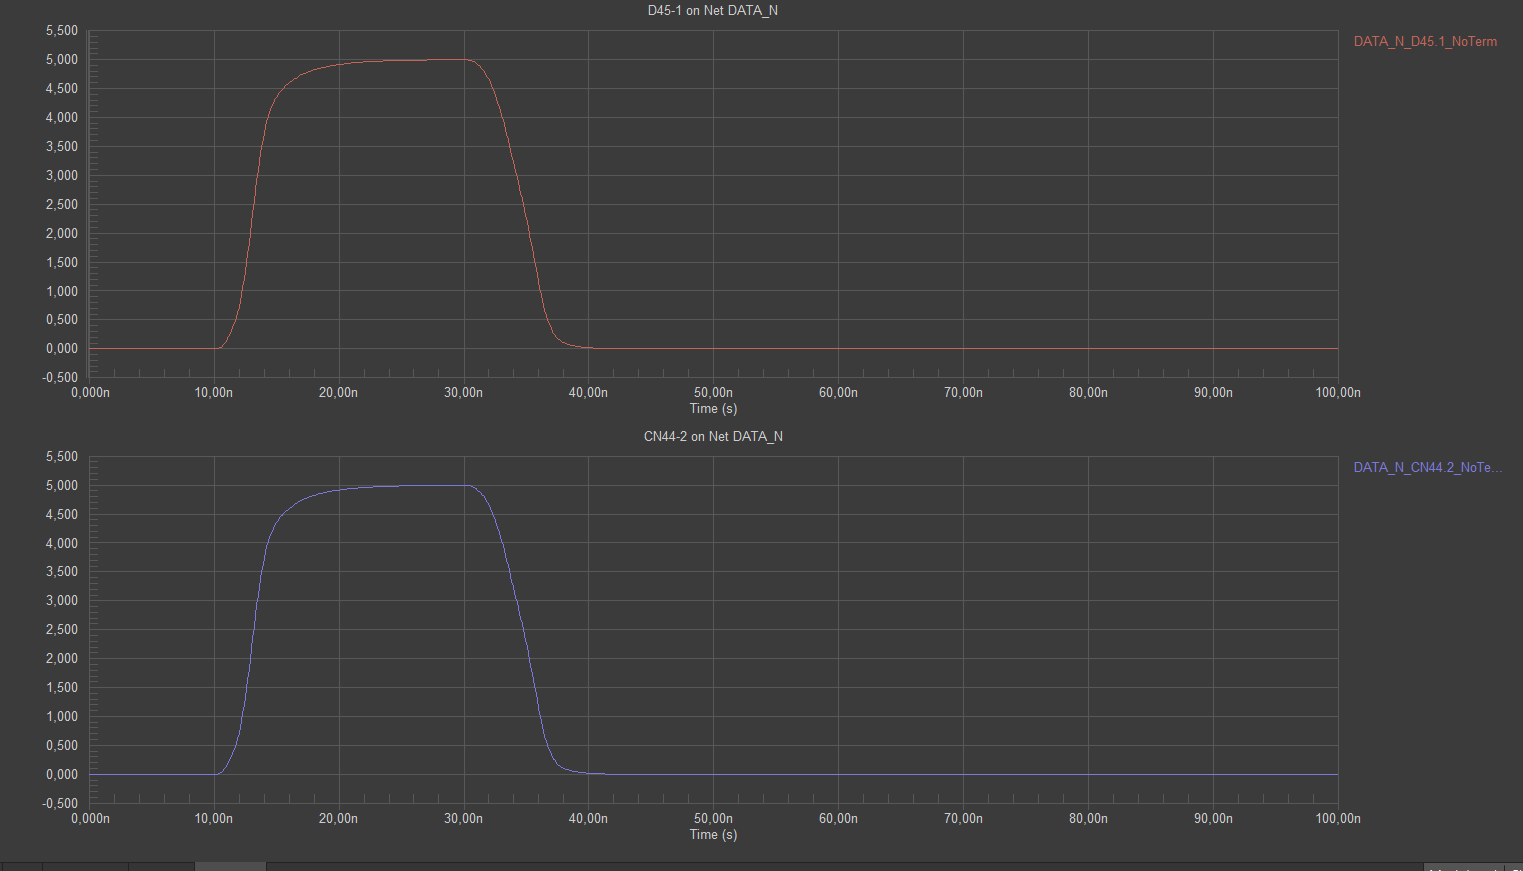
\includegraphics[width=1\linewidth]{Imagenes/Data_reflexions.png}
    \caption{USB}
    \label{fig:reflexiones_usb}
\end{figure}

Aquí se muestra el análisis del USB, como se muestra en la imagen las 2 señales se encuentran perfectas sin aparente distorsión ni sobreoscilaciones.


\subsection{Ethernet}

\begin{figure}[H]
    \centering
    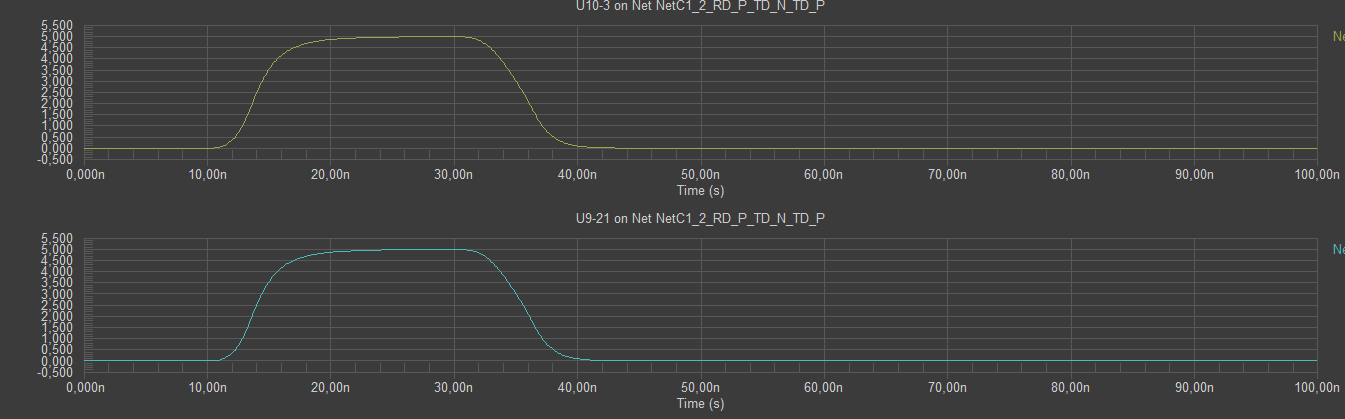
\includegraphics[width=1\linewidth]{Imagenes/ether_con_UWU.png}
    \caption{Ethernet}
    \label{fig:reflexiones_ethernet}
\end{figure}

Aquí se muestra el análisis del USB, como se muestra en la imagen las 2 señales del ethernet, se encuentran perfectas sin aparente distorsión ni sobreoscilaciones.

\end{document}
